% https://tikz.net/neural_networks/

% Author: Izaak Neutelings (September 2021)
% Inspiration:
%   https://www.asimovinstitute.org/neural-network-zoo/
%   https://www.youtube.com/watch?v=aircAruvnKk&list=PLZHQObOWTQDNU6R1_67000Dx_ZCJB-3pi&index=1
\documentclass[border=3pt,tikz]{standalone}
\usepackage{amsmath} % for aligned
%\usepackage{amssymb} % for \mathbb
\usepackage{tikz}
%\usepackage{etoolbox} % for \ifthen
\usepackage{listofitems} % for \readlist to create arrays
\usetikzlibrary{arrows.meta} % for arrow size
\usepackage[outline]{contour} % glow around text
\contourlength{1.4pt}

\tikzset{>=latex} % for LaTeX arrow head
\usepackage{xcolor}
\colorlet{myred}{red!80!black}
\colorlet{myblue}{blue!80!black}
\colorlet{mygreen}{green!60!black}
\colorlet{myorange}{orange!70!red!60!black}
\colorlet{mydarkred}{red!30!black}
\colorlet{mydarkblue}{blue!40!black}
\colorlet{mydarkgreen}{green!30!black}
\tikzstyle{node}=[thick,circle,draw=myblue,minimum size=22,inner sep=0.5,outer sep=0.6]
\tikzstyle{node in}=[node,green!20!black,draw=mygreen!30!black,fill=mygreen!25]
\tikzstyle{node hidden}=[node,blue!20!black,draw=myblue!30!black,fill=myblue!20]
\tikzstyle{node convol}=[node,orange!20!black,draw=myorange!30!black,fill=myorange!20]
\tikzstyle{node out}=[node,red!20!black,draw=myred!30!black,fill=myred!20]
\tikzstyle{connect}=[thick,mydarkblue] %,line cap=round
\tikzstyle{connect arrow}=[-{Latex[length=4,width=3.5]},thick,mydarkblue,shorten <=0.5,shorten >=1]
\tikzset{ % node styles, numbered for easy mapping with \nstyle
  node 1/.style={node in},
  node 2/.style={node hidden},
  node 3/.style={node out},
}
\def\nstyle{int(\lay<\Nnodlen?min(2,\lay):3)} % map layer number onto 1, 2, or 3

\begin{document}


% NEURAL NETWORK with coefficients, arrows
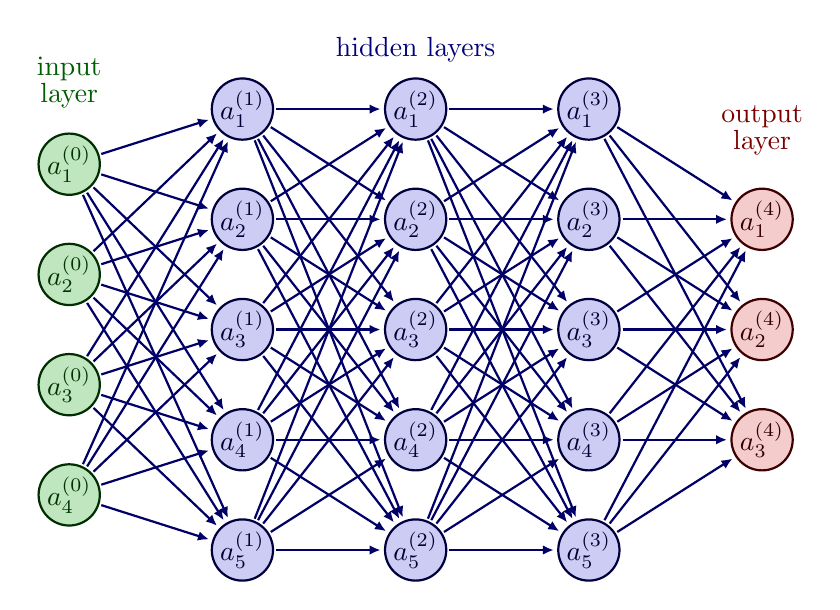
\begin{tikzpicture}[x=2.2cm,y=1.4cm]
  \message{^^JNeural network with arrows}
  \readlist\Nnod{4,5,5,5,3} % array of number of nodes per layer

  \message{^^J  Layer}
  \foreachitem \N \in \Nnod{ % loop over layers
    \edef\lay{\Ncnt} % alias of index of current layer
    \message{\lay,}
    \pgfmathsetmacro\prev{int(\Ncnt-1)} % number of previous layer
    \foreach \i [evaluate={\y=\N/2-\i; \x=\lay; \n=\nstyle;}] in {1,...,\N}{ % loop over nodes

      % NODES
      \node[node \n] (N\lay-\i) at (\x,\y) {$a_\i^{(\prev)}$};
      %\node[circle,inner sep=2] (N\lay-\i') at (\x-0.15,\y) {}; % shifted node
      %\draw[node] (N\lay-\i) circle (\R);

      % CONNECTIONS
      \ifnum\lay>1 % connect to previous layer
        \foreach \j in {1,...,\Nnod[\prev]}{ % loop over nodes in previous layer
          \draw[connect arrow] (N\prev-\j) -- (N\lay-\i); % connect arrows directly
          %\draw[connect arrow] (N\prev-\j) -- (N\lay-\i'); % connect arrows to shifted node
        }
      \fi % else: nothing to connect first layer

    }

  }

  % LABELS
  \node[above=5,align=center,mygreen!60!black] at (N1-1.90) {input\\[-0.2em]layer};
  \node[above=2,align=center,myblue!60!black] at (N3-1.90) {hidden layers};
  \node[above=8,align=center,myred!60!black] at (N\Nnodlen-1.90) {output\\[-0.2em]layer};

\end{tikzpicture}


%% NEURAL NETWORK using \foreach's remember instead of \readlist
%\begin{tikzpicture}[x=2.2cm,y=1.4cm]
%  \message{^^JNeural network with arrows}
%  \def\Ntot{5} % total number of indices
%  \def\nstyle{int(\lay<\Ntot?min(2,\lay):3)} % map layer number onto 1, 2, or 3
%
%  \message{^^J  Layer}
%  \foreach \N [count=\lay,remember={\N as \Nprev (initially 0);}]
%               in {4,5,5,5,3}{ % loop over layers
%    \message{\lay,}
%    \foreach \i [evaluate={\y=\N/2-\i; \x=\lay; \n=\nstyle; \prev=int(\lay-1);}]
%                 in {1,...,\N}{ % loop over nodes
%      \node[node \n] (N\lay-\i) at (\x,\y) {$a_\i^{(\prev)}$};
%
%      % CONNECTIONS
%      \ifnum\Nprev>0 % connect to previous layer
%        \foreach \j in {1,...,\Nprev}{ % loop over nodes in previous layer
%          \draw[connect arrow] (N\prev-\j) -- (N\lay-\i); % connect arrows directly
%        }
%      \fi
%
%    }
%  }
%
%  % LABELS
%  \node[above=5,align=center,mygreen!60!black] at (N1-1.90) {input\\[-0.2em]layer};
%  \node[above=2,align=center,myblue!60!black] at (N3-1.90) {hidden layers};
%  \node[above=8,align=center,myred!60!black] at (N\Ntot-1.90) {output\\[-0.2em]layer};
%
%\end{tikzpicture}


% NEURAL NETWORK with coefficients, uniform arrows
\newcommand\setAngles[3]{
  \pgfmathanglebetweenpoints{\pgfpointanchor{#2}{center}}{\pgfpointanchor{#1}{center}}
  \pgfmathsetmacro\angmin{\pgfmathresult}
  \pgfmathanglebetweenpoints{\pgfpointanchor{#2}{center}}{\pgfpointanchor{#3}{center}}
  \pgfmathsetmacro\angmax{\pgfmathresult}
  \pgfmathsetmacro\dang{\angmax-\angmin}
  \pgfmathsetmacro\dang{\dang<0?\dang+360:\dang}
}
\begin{tikzpicture}[x=2.2cm,y=1.4cm]
  \message{^^JNeural network with uniform arrows}
  \readlist\Nnod{4,5,5,5,3} % array of number of nodes per layer

  \foreachitem \N \in \Nnod{ % loop over layers
    \def\lay{\Ncnt} % alias of index of current layer
    \pgfmathsetmacro\prev{int(\Ncnt-1)} % number of previous layer
    \foreach \i [evaluate={\y=\N/2-\i; \x=\lay; \n=\nstyle;}] in {1,...,\N}{ % loop over nodes

      % NODES
      \node[node \n] (N\lay-\i) at (\x,\y) {$a_\i^{(\prev)}$};

      % CONNECTIONS
      \ifnum\lay>1 % connect to previous layer
        \setAngles{N\prev-1}{N\lay-\i}{N\prev-\Nnod[\prev]} % angles in current node
        %\draw[red,thick] (N\lay-\i)++(\angmin:0.2) --++ (\angmin:-0.5) node[right,scale=0.5] {\dang};
        %\draw[blue,thick] (N\lay-\i)++(\angmax:0.2) --++ (\angmax:-0.5) node[right,scale=0.5] {\angmin, \angmax};
        \foreach \j [evaluate={\ang=\angmin+\dang*(\j-1)/(\Nnod[\prev]-1);}] %-180+(\angmax-\angmin)*\j/\Nnod[\prev]
                    in {1,...,\Nnod[\prev]}{ % loop over nodes in previous layer
          \setAngles{N\lay-1}{N\prev-\j}{N\lay-\N} % angles out from previous node
          \pgfmathsetmacro\angout{\angmin+(\dang-360)*(\i-1)/(\N-1)} % number of previous layer
          %\draw[connect arrow,white,line width=1.1] (N\prev-\j.{\angout}) -- (N\lay-\i.{\ang});
          \draw[connect arrow] (N\prev-\j.{\angout}) -- (N\lay-\i.{\ang}); % connect arrows uniformly
        }
      \fi % else: nothing to connect first layer

    }
  }

  % LABELS
  \node[above=5,align=center,mygreen!60!black] at (N1-1.90) {input\\[-0.2em]layer};
  \node[above=2,align=center,myblue!60!black] at (N3-1.90) {hidden layers};
  \node[above=8,align=center,myred!60!black] at (N\Nnodlen-1.90) {output\\[-0.2em]layer};

\end{tikzpicture}


% NEURAL NETWORK with coefficients, no arrows
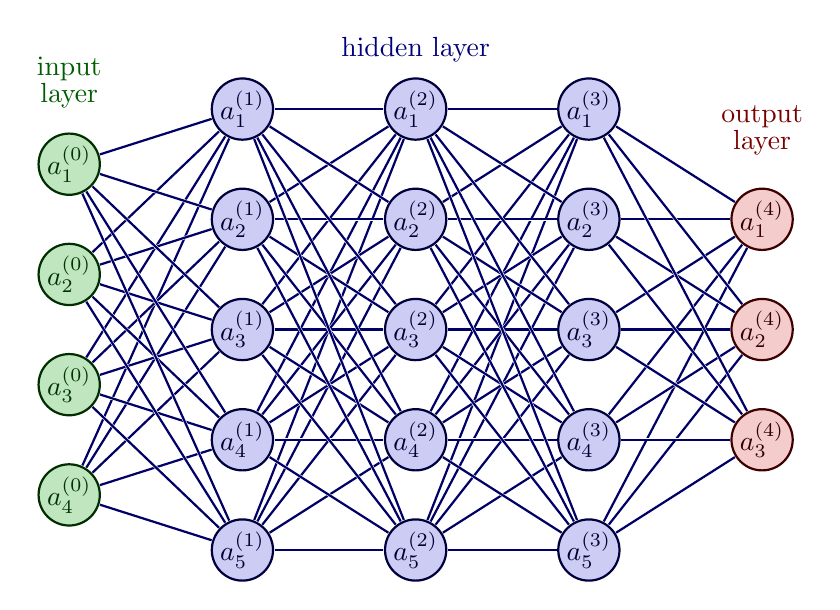
\begin{tikzpicture}[x=2.2cm,y=1.4cm]
  \message{^^JNeural network without arrows}
  \readlist\Nnod{4,5,5,5,3} % array of number of nodes per layer

  \message{^^J  Layer}
  \foreachitem \N \in \Nnod{ % loop over layers
    \def\lay{\Ncnt} % alias of index of current layer
    \pgfmathsetmacro\prev{int(\Ncnt-1)} % number of previous layer
    \message{\lay,}
    \foreach \i [evaluate={\y=\N/2-\i; \x=\lay; \n=\nstyle;}] in {1,...,\N}{ % loop over nodes

      % NODES
      \node[node \n] (N\lay-\i) at (\x,\y) {$a_\i^{(\prev)}$};

      % CONNECTIONS
      \ifnum\lay>1 % connect to previous layer
        \foreach \j in {1,...,\Nnod[\prev]}{ % loop over nodes in previous layer
          \draw[connect,white,line width=1.2] (N\prev-\j) -- (N\lay-\i);
          \draw[connect] (N\prev-\j) -- (N\lay-\i);
          %\draw[connect] (N\prev-\j.0) -- (N\lay-\i.180); % connect to left
        }
      \fi % else: nothing to connect first layer

    }
  }

  % LABELS
  \node[above=5,align=center,mygreen!60!black] at (N1-1.90) {input\\[-0.2em]layer};
  \node[above=2,align=center,myblue!60!black] at (N3-1.90) {hidden layer};
  \node[above=8,align=center,myred!60!black] at (N\Nnodlen-1.90) {output\\[-0.2em]layer};

\end{tikzpicture}


% NEURAL NETWORK with coefficients, shifted
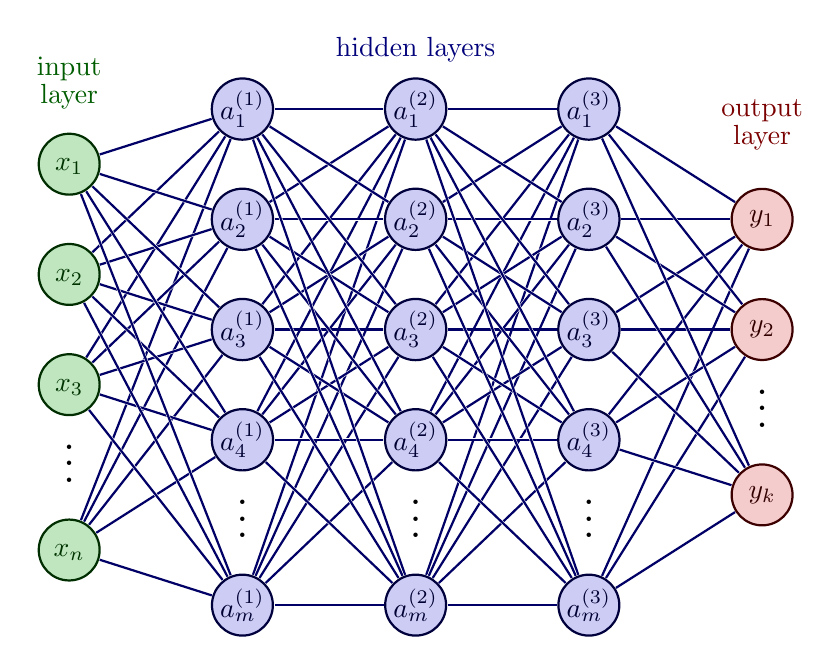
\begin{tikzpicture}[x=2.2cm,y=1.4cm]
  \message{^^JNeural network, shifted}
  \readlist\Nnod{4,5,5,5,3} % array of number of nodes per layer
  \readlist\Nstr{n,m,m,m,k} % array of string number of nodes per layer
  \readlist\Cstr{\strut x,a^{(\prev)},a^{(\prev)},a^{(\prev)},y} % array of coefficient symbol per layer
  \def\yshift{0.5} % shift last node for dots

  \message{^^J  Layer}
  \foreachitem \N \in \Nnod{ % loop over layers
    \def\lay{\Ncnt} % alias of index of current layer
    \pgfmathsetmacro\prev{int(\Ncnt-1)} % number of previous layer
    \message{\lay,}
    \foreach \i [evaluate={\c=int(\i==\N); \y=\N/2-\i-\c*\yshift;
                 \index=(\i<\N?int(\i):"\Nstr[\lay]");
                 \x=\lay; \n=\nstyle;}] in {1,...,\N}{ % loop over nodes
      % NODES
      \node[node \n] (N\lay-\i) at (\x,\y) {$\Cstr[\lay]_{\index}$};

      % CONNECTIONS
      \ifnum\lay>1 % connect to previous layer
        \foreach \j in {1,...,\Nnod[\prev]}{ % loop over nodes in previous layer
          \draw[connect,white,line width=1.2] (N\prev-\j) -- (N\lay-\i);
          \draw[connect] (N\prev-\j) -- (N\lay-\i);
          %\draw[connect] (N\prev-\j.0) -- (N\lay-\i.180); % connect to left
        }
      \fi % else: nothing to connect first layer

    }
    \path (N\lay-\N) --++ (0,1+\yshift) node[midway,scale=1.5] {$\vdots$};
  }

  % LABELS
  \node[above=5,align=center,mygreen!60!black] at (N1-1.90) {input\\[-0.2em]layer};
  \node[above=2,align=center,myblue!60!black] at (N3-1.90) {hidden layers};
  \node[above=10,align=center,myred!60!black] at (N\Nnodlen-1.90) {output\\[-0.2em]layer};

\end{tikzpicture}


% NEURAL NETWORK no text
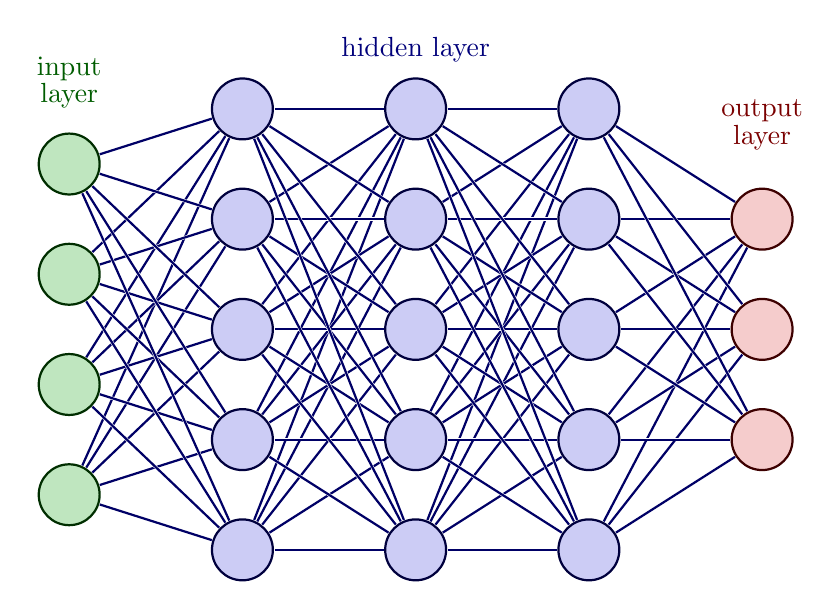
\begin{tikzpicture}[x=2.2cm,y=1.4cm]
  \message{^^JNeural network without text}
  \readlist\Nnod{4,5,5,5,3} % array of number of nodes per layer

  \message{^^J  Layer}
  \foreachitem \N \in \Nnod{ % loop over layers
    \def\lay{\Ncnt} % alias of index of current layer
    \pgfmathsetmacro\prev{int(\Ncnt-1)} % number of previous layer
    \message{\lay,}
    \foreach \i [evaluate={\y=\N/2-\i; \x=\lay; \n=\nstyle;}] in {1,...,\N}{ % loop over nodes

      % NODES
      \node[node \n] (N\lay-\i) at (\x,\y) {};

      % CONNECTIONS
      \ifnum\lay>1 % connect to previous layer
        \foreach \j in {1,...,\Nnod[\prev]}{ % loop over nodes in previous layer
          \draw[connect,white,line width=1.2] (N\prev-\j) -- (N\lay-\i);
          \draw[connect] (N\prev-\j) -- (N\lay-\i);
          %\draw[connect] (N\prev-\j.0) -- (N\lay-\i.180); % connect to left
        }
      \fi % else: nothing to connect first layer

    }
  }

  % LABELS
  \node[above=5,align=center,mygreen!60!black] at (N1-1.90) {input\\[-0.2em]layer};
  \node[above=2,align=center,myblue!60!black] at (N3-1.90) {hidden layer};
  \node[above=10,align=center,myred!60!black] at (N\Nnodlen-1.90) {output\\[-0.2em]layer};

\end{tikzpicture}


% NEURAL NETWORK no text - large
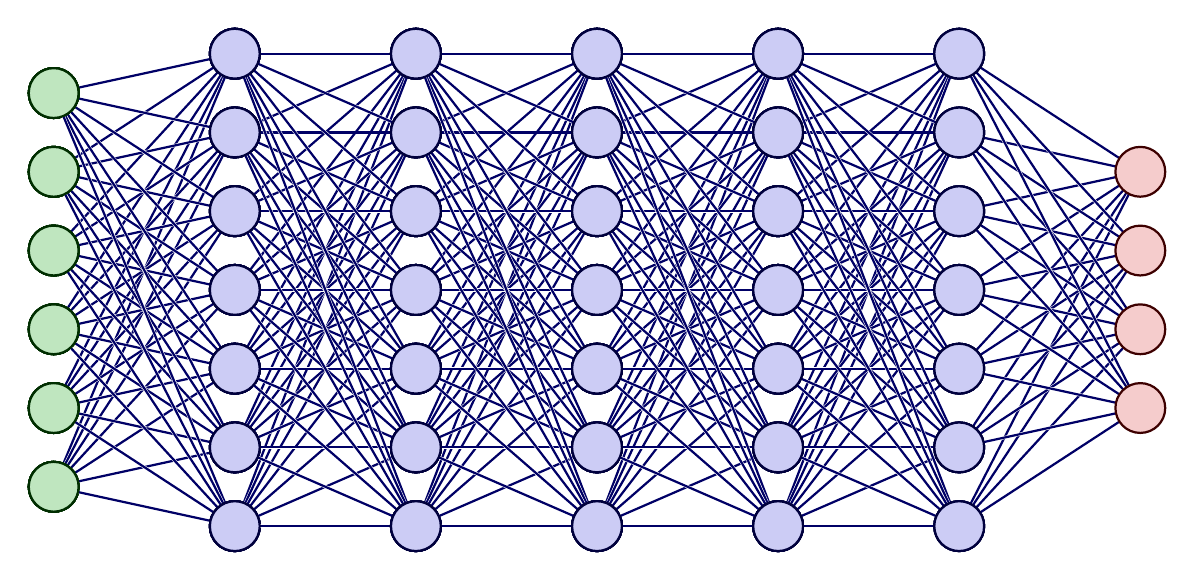
\begin{tikzpicture}[x=2.3cm,y=1.0cm]
  \message{^^JNeural network large}
  \readlist\Nnod{6,7,7,7,7,7,4} % array of number of nodes per layer

  \message{^^J  Layer}
  \foreachitem \N \in \Nnod{ % loop over layers
    \def\lay{\Ncnt} % alias of index of current layer
    \pgfmathsetmacro\prev{int(\Ncnt-1)} % number of previous layer
    \message{\lay,}
    \foreach \i [evaluate={\y=\N/2-\i; \x=\lay; \n=\nstyle;
                           \nprev=int(\prev<\Nnodlen?min(2,\prev):3);}] in {1,...,\N}{ % loop over nodes

      % NODES
      %\node[node \n,outer sep=0.6,minimum size=18] (N\lay-\i) at (\x,\y) {};
      \coordinate (N\lay-\i) at (\x,\y);

      % CONNECTIONS
      \ifnum\lay>1 % connect to previous layer
        \foreach \j in {1,...,\Nnod[\prev]}{ % loop over nodes in previous layer
          \draw[connect,white,line width=1.2] (N\prev-\j) -- (N\lay-\i);
          \draw[connect] (N\prev-\j) -- (N\lay-\i);
          %\draw[connect] (N\prev-\j.0) -- (N\lay-\i.180); % connect to left
          \node[node \nprev,minimum size=18] at (N\prev-\j) {}; % draw node over lines
        }
        \ifnum \lay=\Nnodlen % draw last node over lines
          \node[node \n,minimum size=18] at (N\lay-\i) {};
        \fi
      \fi % else: nothing to connect first layer

    }
  }

\end{tikzpicture}


% DEEP CONVOLUTIONAL NEURAL NETWORK
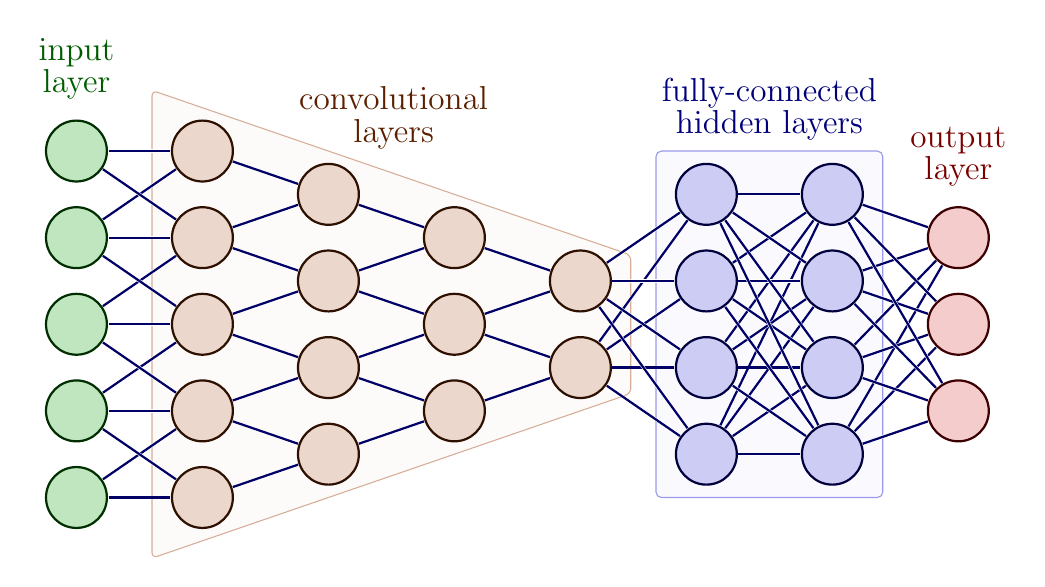
\begin{tikzpicture}[x=1.6cm,y=1.1cm]
  \large
  \message{^^JDeep convolution neural network}
  \readlist\Nnod{5,5,4,3,2,4,4,3} % array of number of nodes per layer
  \def\NC{6} % number of convolutional layers
  \def\nstyle{int(\lay<\Nnodlen?(\lay<\NC?min(2,\lay):3):4)} % map layer number on 1, 2, or 3
  \tikzset{ % node styles, numbered for easy mapping with \nstyle
    node 1/.style={node in},
    node 2/.style={node convol},
    node 3/.style={node hidden},
    node 4/.style={node out},
  }

  % TRAPEZIA
  \draw[myorange!40,fill=myorange,fill opacity=0.02,rounded corners=2]
    %(1.6,-2.5) rectangle (4.4,2.5);
    (1.6,-2.7) --++ (0,5.4) --++ (3.8,-1.9) --++ (0,-1.6) -- cycle;
  \draw[myblue!40,fill=myblue,fill opacity=0.02,rounded corners=2]
    (5.6,-2.0) rectangle++ (1.8,4.0);
  \node[right=19,above=3,align=center,myorange!60!black] at (3.1,1.8) {convolutional\\[-0.2em]layers};
  \node[above=3,align=center,myblue!60!black] at (6.5,1.9) {fully-connected\\[-0.2em]hidden layers};

  \message{^^J  Layer}
  \foreachitem \N \in \Nnod{ % loop over layers
    \def\lay{\Ncnt} % alias of index of current layer
    \pgfmathsetmacro\prev{int(\Ncnt-1)} % number of previous layer
    %\pgfmathsetmacro\Nprev{\Nnod[\prev]} % array of number of nodes in previous layer
    \message{\lay,}
    \foreach \i [evaluate={\y=\N/2-\i+0.5; \x=\lay; \n=\nstyle;}] in {1,...,\N}{ % loop over nodes
      %\message{^^J  Layer \lay, node \i}

      % NODES
      \node[node \n,outer sep=0.6] (N\lay-\i) at (\x,\y) {};

      % CONNECTIONS
      \ifnum\lay>1 % connect to previous layer
        \ifnum\lay<\NC % convolutional layers
          \foreach \j [evaluate={\jprev=int(\i-\j); \cconv=int(\Nnod[\prev]>\N); \ctwo=(\cconv&&\j>0);
                       \c=int((\jprev<1||\jprev>\Nnod[\prev]||\ctwo)?0:1);}]
                       in {-1,0,1}{
            \ifnum\c=1
              \ifnum\cconv=0
                \draw[connect,white,line width=1.2] (N\prev-\jprev) -- (N\lay-\i);
              \fi
              \draw[connect] (N\prev-\jprev) -- (N\lay-\i);
            \fi
          }

        \else % fully connected layers
          \foreach \j in {1,...,\Nnod[\prev]}{ % loop over nodes in previous layer
            \draw[connect,white,line width=1.2] (N\prev-\j) -- (N\lay-\i);
            \draw[connect] (N\prev-\j) -- (N\lay-\i);
          }
        \fi
      \fi % else: nothing to connect first layer

    }
  }

  % LABELS
  \node[above=3,align=center,mygreen!60!black] at (N1-1.90) {input\\[-0.2em]layer};
  \node[above=3,align=center,myred!60!black] at (N\Nnodlen-1.90) {output\\[-0.2em]layer};

\end{tikzpicture}


% AUTOENCODER
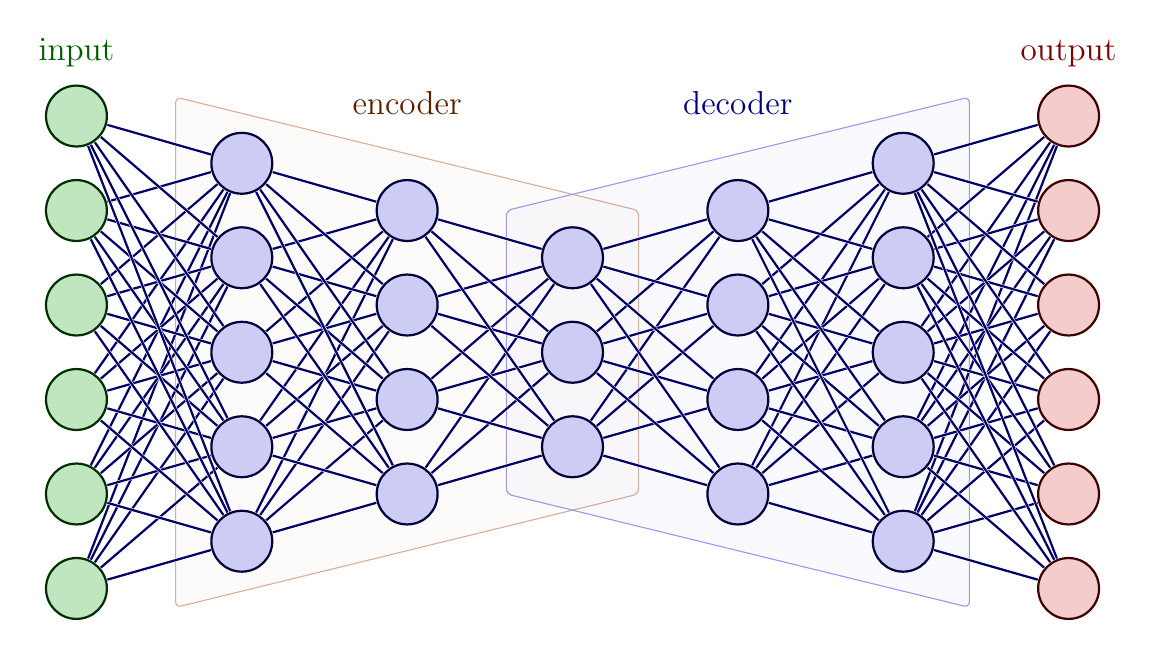
\begin{tikzpicture}[x=2.1cm,y=1.2cm]
  \large
  \message{^^JNeural network without arrows}
  \readlist\Nnod{6,5,4,3,4,5,6} % array of number of nodes per layer

  % TRAPEZIA
  \node[above,align=center,myorange!60!black] at (3,2.4) {encoder};
  \node[above,align=center,myblue!60!black] at (5,2.4) {decoder};
  \draw[myorange!40,fill=myorange,fill opacity=0.02,rounded corners=2]
    (1.6,-2.7) --++ (0,5.4) --++ (2.8,-1.2) --++ (0,-3) -- cycle;
  \draw[myblue!40,fill=myblue,fill opacity=0.02,rounded corners=2]
    (6.4,-2.7) --++ (0,5.4) --++ (-2.8,-1.2) --++ (0,-3) -- cycle;

  \message{^^J  Layer}
  \foreachitem \N \in \Nnod{ % loop over layers
    \def\lay{\Ncnt} % alias of index of current layer
    \pgfmathsetmacro\prev{int(\Ncnt-1)} % number of previous layer
    \message{\lay,}
    \foreach \i [evaluate={\y=\N/2-\i+0.5; \x=\lay; \n=\nstyle;}] in {1,...,\N}{ % loop over nodes

      % NODES
      \node[node \n,outer sep=0.6] (N\lay-\i) at (\x,\y) {};

      % CONNECTIONS
      \ifnum\lay>1 % connect to previous layer
        \foreach \j in {1,...,\Nnod[\prev]}{ % loop over nodes in previous layer
          \draw[connect,white,line width=1.2] (N\prev-\j) -- (N\lay-\i);
          \draw[connect] (N\prev-\j) -- (N\lay-\i);
          %\draw[connect] (N\prev-\j.0) -- (N\lay-\i.180); % connect to left
        }
      \fi % else: nothing to connect first layer

    }
  }

  % LABELS
  \node[above=2,align=center,mygreen!60!black] at (N1-1.90) {input};
  \node[above=2,align=center,myred!60!black] at (N\Nnodlen-1.90) {output};

\end{tikzpicture}


% NEURAL NETWORK activation
% https://www.youtube.com/watch?v=aircAruvnKk&list=PLZHQObOWTQDNU6R1_67000Dx_ZCJB-3pi&index=1
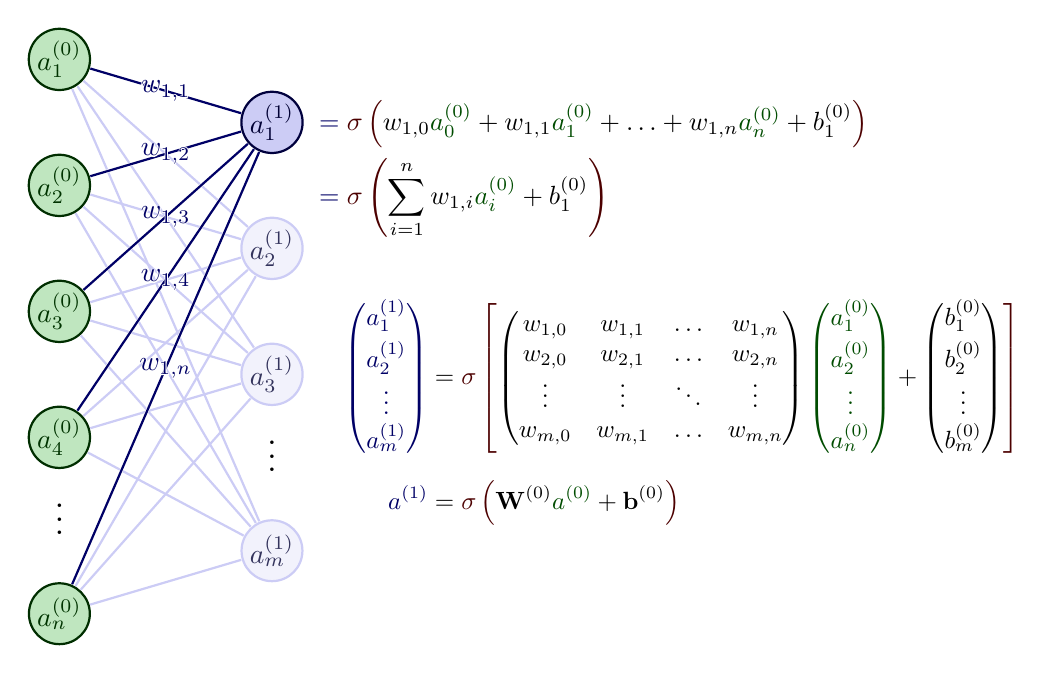
\begin{tikzpicture}[x=2.7cm,y=1.6cm]
  \message{^^JNeural network activation}
  \def\NI{5} % number of nodes in input layers
  \def\NO{4} % number of nodes in output layers
  \def\yshift{0.4} % shift last node for dots

  % INPUT LAYER
  \foreach \i [evaluate={\c=int(\i==\NI); \y=\NI/2-\i-\c*\yshift; \index=(\i<\NI?int(\i):"n");}]
              in {1,...,\NI}{ % loop over nodes
    \node[node in,outer sep=0.6] (NI-\i) at (0,\y) {$a_{\index}^{(0)}$};
  }

  % OUTPUT LAYER
  \foreach \i [evaluate={\c=int(\i==\NO); \y=\NO/2-\i-\c*\yshift; \index=(\i<\NO?int(\i):"m");}]
    in {\NO,...,1}{ % loop over nodes
    \ifnum\i=1 % high-lighted node
      \node[node hidden]
        (NO-\i) at (1,\y) {$a_{\index}^{(1)}$};
      \foreach \j [evaluate={\index=(\j<\NI?int(\j):"n");}] in {1,...,\NI}{ % loop over nodes in previous layer
        \draw[connect,white,line width=1.2] (NI-\j) -- (NO-\i);
        \draw[connect] (NI-\j) -- (NO-\i)
          node[pos=0.50] {\contour{white}{$w_{1,\index}$}};
      }
    \else % other light-colored nodes
      \node[node,blue!20!black!80,draw=myblue!20,fill=myblue!5]
        (NO-\i) at (1,\y) {$a_{\index}^{(1)}$};
      \foreach \j in {1,...,\NI}{ % loop over nodes in previous layer
        %\draw[connect,white,line width=1.2] (NI-\j) -- (NO-\i);
        \draw[connect,myblue!20] (NI-\j) -- (NO-\i);
      }
    \fi
  }

  % DOTS
  \path (NI-\NI) --++ (0,1+\yshift) node[midway,scale=1.2] {$\vdots$};
  \path (NO-\NO) --++ (0,1+\yshift) node[midway,scale=1.2] {$\vdots$};

  % EQUATIONS
  \def\agr#1{{\color{mydarkgreen}a_{#1}^{(0)}}}
  \node[below=17,right=11,mydarkblue,scale=0.95] at (NO-1)
    {$\begin{aligned} %\underset{\text{bias}}{b_1}
       &= \color{mydarkred}\sigma\left( \color{black}
            w_{1,0}\agr{0} + w_{1,1}\agr{1} + \ldots + w_{1,n}\agr{n} + b_1^{(0)}
          \color{mydarkred}\right)\\
       &= \color{mydarkred}\sigma\left( \color{black}
            \sum_{i=1}^{n} w_{1,i}\agr{i} + b_1^{(0)}
           \color{mydarkred}\right)
     \end{aligned}$};
  \node[right,scale=0.9] at (1.3,-1.3)
    {$\begin{aligned}
      {\color{mydarkblue}
      \begin{pmatrix}
        a_{1}^{(1)} \\[0.3em]
        a_{2}^{(1)} \\
        \vdots \\
        a_{m}^{(1)}
      \end{pmatrix}}
      &=
      \color{mydarkred}\sigma\left[ \color{black}
      \begin{pmatrix}
        w_{1,0} & w_{1,1} & \ldots & w_{1,n} \\
        w_{2,0} & w_{2,1} & \ldots & w_{2,n} \\
        \vdots  & \vdots  & \ddots & \vdots  \\
        w_{m,0} & w_{m,1} & \ldots & w_{m,n}
      \end{pmatrix}
      {\color{mydarkgreen}
      \begin{pmatrix}
        a_{1}^{(0)} \\[0.3em]
        a_{2}^{(0)} \\
        \vdots \\
        a_{n}^{(0)}
      \end{pmatrix}}
      +
      \begin{pmatrix}
        b_{1}^{(0)} \\[0.3em]
        b_{2}^{(0)} \\
        \vdots \\
        b_{m}^{(0)}
      \end{pmatrix}
      \color{mydarkred}\right]\\[0.5em]
      {\color{mydarkblue}a^{(1)}}
      &= \color{mydarkred}\sigma\left( \color{black}
           \mathbf{W}^{(0)} {\color{mydarkgreen}a^{(0)}}+\mathbf{b}^{(0)}
         \color{mydarkred}\right)
         %\color{black},\quad \mathbf{W}^{(0)} \in \mathbb{R}^{m\times n}
    \end{aligned}$};

\end{tikzpicture}


\end{document}
